\thispagestyle{doisongtoanhocnone}
\pagestyle{doisongtoanhoc}
\everymath{\color{doisongtoanhoc}}
\graphicspath{{../doisongtoanhoc/pic/}}
\blfootnote{$^1$\color{doisongtoanhoc}Trung tâm Thông tin -- Tư liệu, Viện Hàn lâm Khoa học và Công nghệ Việt Nam.}
\begingroup
\AddToShipoutPicture*{\put(0,616){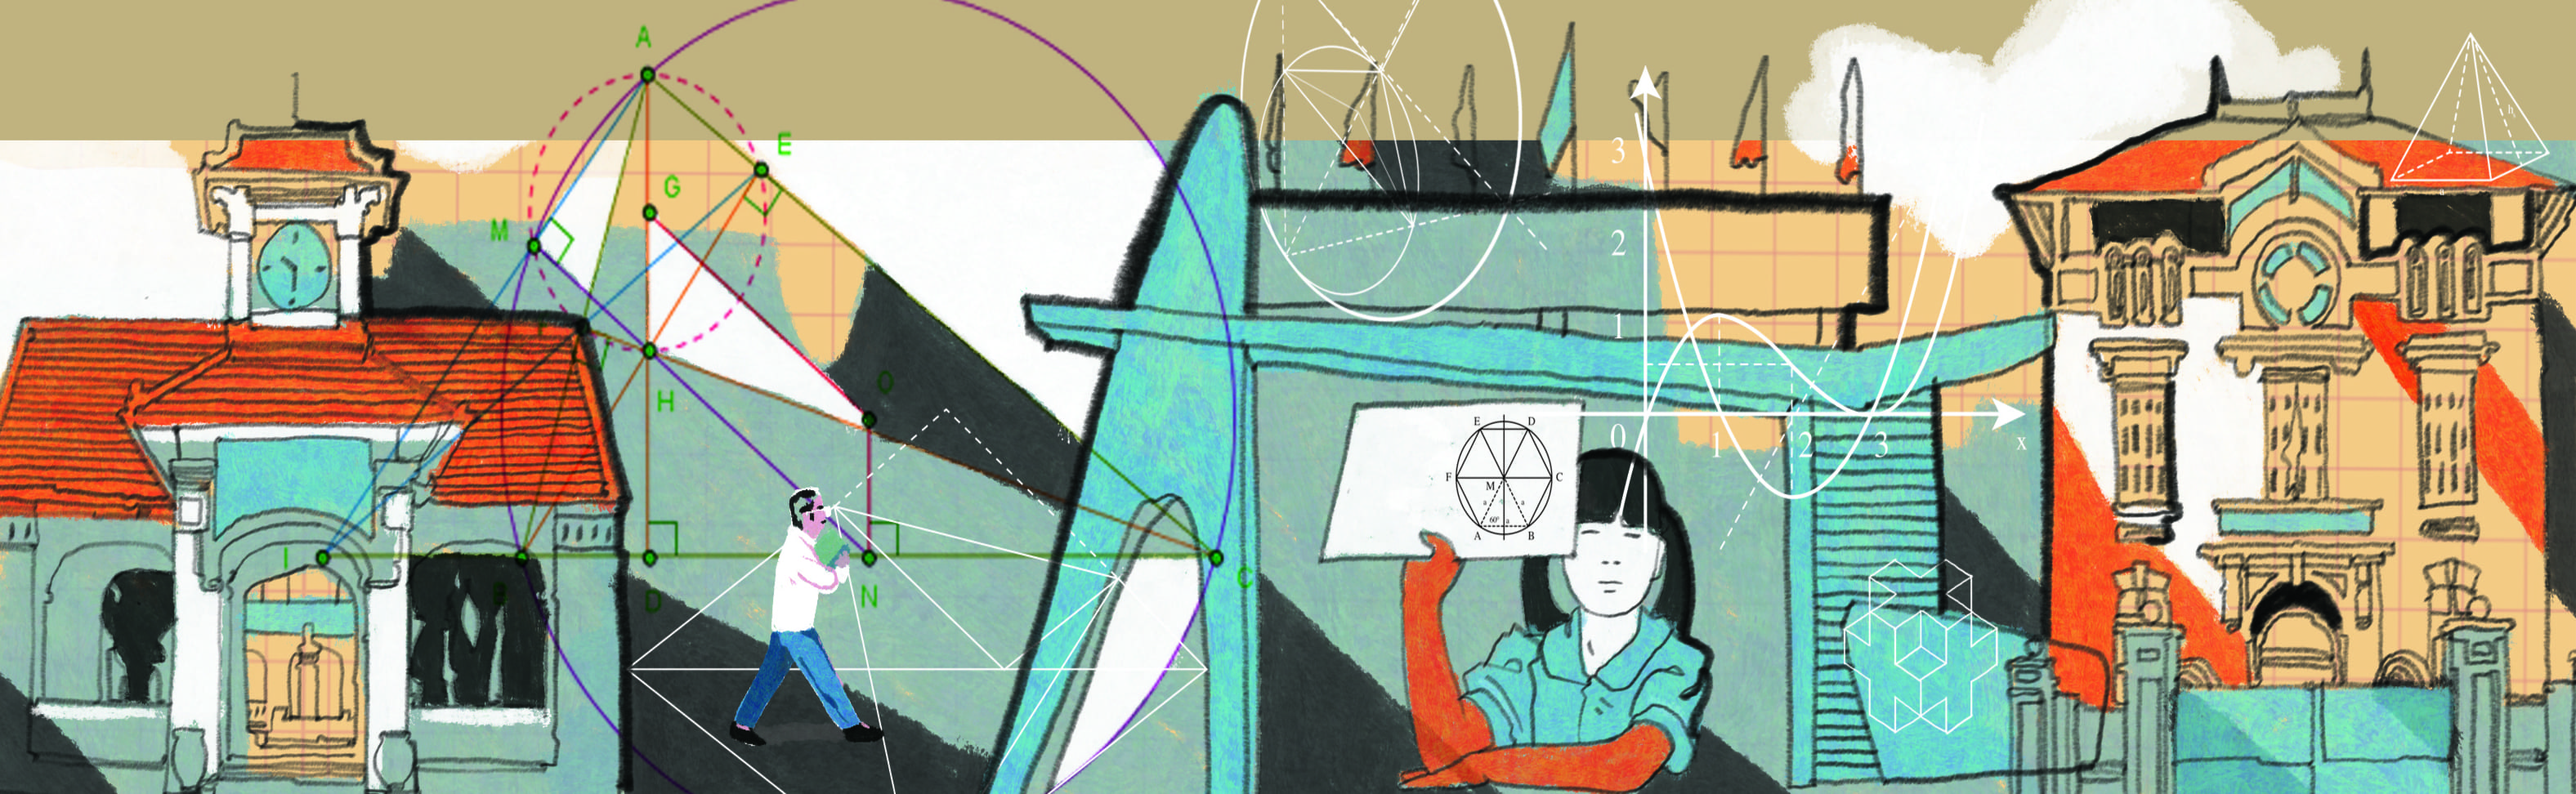
\includegraphics[width=19.3cm]{../bannerdoisong}}}
\AddToShipoutPicture*{\put(80,522){
\includegraphics[scale=1]{../tieude.pdf}}}\centering
\endgroup

\vspace*{190pt}


\begin{multicols}{2}	
	\textit{Chiều ngày $14/3/2022$, Trung tâm Quốc tế Đào tạo và Nghiên cứu Toán học UNESCO, Viện Toán học -- Viện Hàn lâm Khoa học và Công nghệ Việt Nam và Quỹ Đổi mới sáng tạo Vingroup đồng tổ chức ngày Toán học quốc tế $2022$ với chủ đề: ``Toán học kết nối chúng ta", nhằm nhấn mạnh sự kết nối và vai trò của của toán học trong không gian và thời gian, toán học liên kết các ngành khoa học và toán học kết nối chúng ta như những nhân tố của xã hội.}
	\begin{figure}[H]
		\centering
		\vspace*{-5pt}
		\captionsetup{labelformat= empty, justification=centering}
		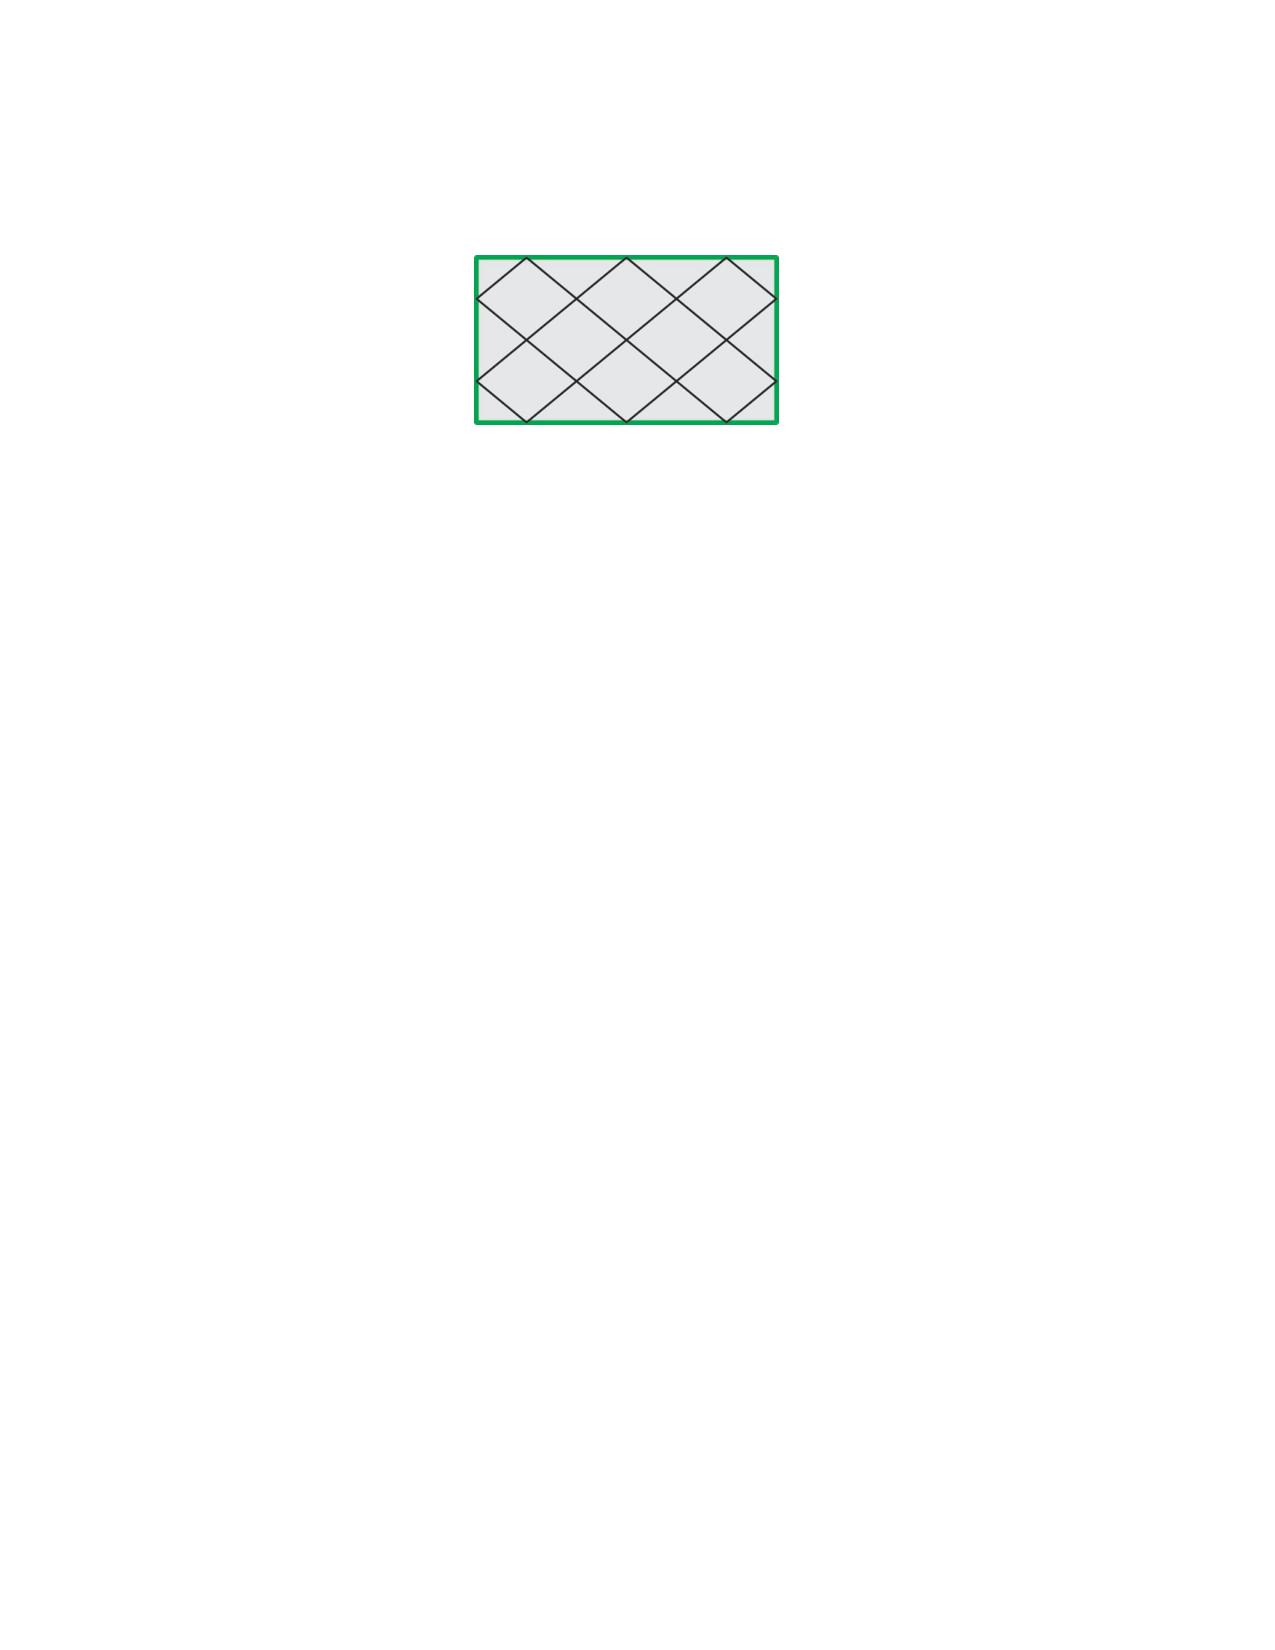
\includegraphics[width=1\linewidth]{1}
		\vspace*{-10pt}
	\end{figure}
	Tại phiên họp lần thứ $40$ của Đại hội đồng UNESCO ngày $26$ tháng $11$ năm $2019$, tổ chức Giáo dục, Khoa học và Văn hóa Liên Hiệp Quốc chính thức tuyên bố ngày $14$ tháng $3$ hằng năm là ngày Toán học Quốc tế (International Day of Mathematics--IDM). Năm $2022$, Unesco đã chọn chủ đề cho Ngày Toán học quốc tế là ``Toán học kết nối" (\textit{Mathematics Unites}) ``bởi vì Toán học là một ngôn ngữ chung để chúng ta tìm đến nhau".
	\vskip 0.1cm
	Trên tinh thần đó, Ngày Toán học quốc tế $2022$ với chủ đề: ``Toán học kết nối chúng ta", đã tạo dấu ấn kết nối liên ngành bằng nội dung của ba bài giảng đại chúng.
	\vskip 0.1cm
	Bài giảng ``Toán học trong nghiên cứu khí hậu và biến đổi khí hậu quy mô khu vực" do PGS. TSKH Ngô Đức Thành -- Đồng Trưởng Khoa Vũ trụ và Ứng dụng, Trường Đại học Khoa học và Công nghệ Hà Nội, Viện Hàn lâm Khoa học và Công nghệ Việt Nam trình bày, đã đặt ra và trả lời $14$ câu hỏi xung quanh các ứng dụng của Toán học trong nghiên cứu biến đổi khí hậu trong vòng $100$ năm nay. Thông qua bài giảng, người nghe thấy được các công thức toán học xuất hiện trong các mô hình tính toán về biến đổi khí hậu như: Mô hình cân bằng năng lượng, mô hình đối lưu khí quyển \ldots 
	\vskip 0.1cm
	Bài giảng ``Giải mã DNA của bạn: lý thuyết đồ thị có thể giúp gì?" do TS. Võ Sỹ Nam -- Giám đốc Trung tâm Tin Y Sinh, Viện Nghiên cứu dữ liệu lớn Vingroup \& Giảng viên liên kết, Vin University trình bày. Kể từ khi dự án giải mã DNA người đầu tiên trên thế giới hoàn tất vào năm $2003$, đã có rất nhiều dự án tiếp theo được thực hiện. Với lượng dữ liệu khổng lồ lên đến hàng petabyte tạo ra từ các dự án này, các phương pháp và công cụ tính toán hiệu quả trở nên tối cần thiết. TS. Võ Sỹ Nam đã chia sẻ về vai trò và ý nghĩa của lý thuyết đồ thị trong giải mã DNA cũng như tiềm năng ứng dụng của lý thuyết này trong di truyền học nói chung.
	\begin{figure}[H]
		\centering
		\vspace*{-5pt}
		\captionsetup{labelformat= empty, justification=centering}
		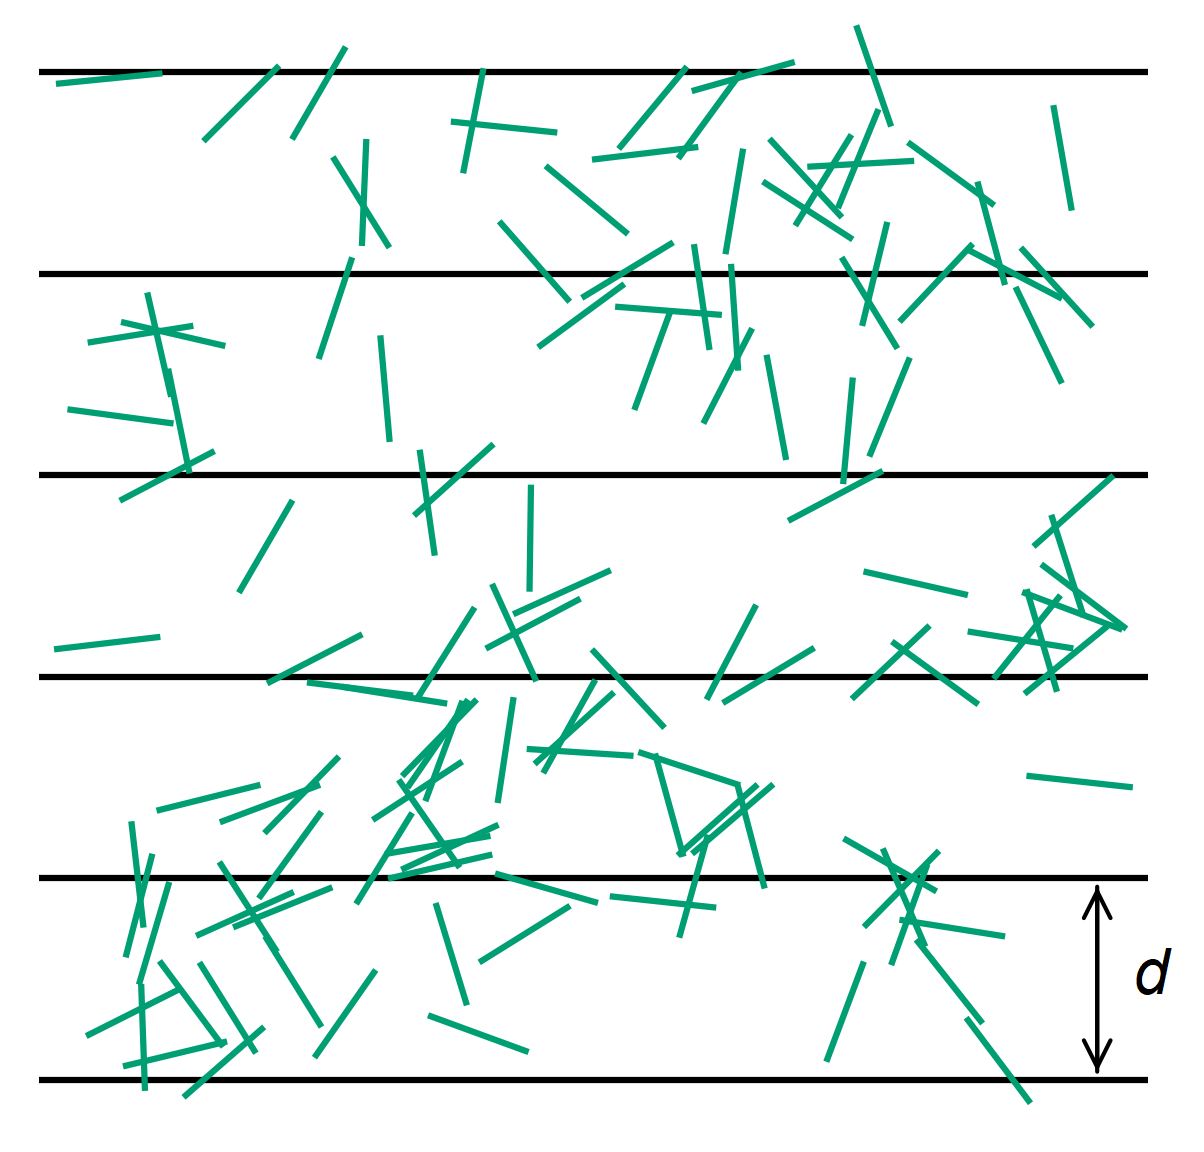
\includegraphics[width=1\linewidth]{2}
		\vspace*{-10pt}
	\end{figure}
	Bài giảng thứ ba, ``Toán là chúng ta", do diễn giả Nguyễn Như Huy -- Giám đốc nghệ thuật của ZeroStation trình bày. Từ góc độ lịch sử triết học, diễn giả Như Huy trao đổi về sự khác biệt giữa toán, xét như một lối suy tư có tính căn nguyên của con người về vật, với toán học, là một trong những hình thái phát triển hiện đại của toán. Diễn giả sử dụng lối suy tư toán nói trên để tiếp cận với các sự vật và hiện tượng phi toán học, như lịch sử nghệ thuật và mối quan hệ giữa quan niệm về logic kiểu Wittgenstein với Tâm, xét như một thực tại của tư tưởng Thiền. 
	\vskip 0.1cm
	Sau các bài giảng là tọa đàm ``Toán học kết nối chúng ta" với những trao đổi xung quanh ứng dụng toán học trong trong khoa học cũng như trong cuộc sống. Với sự góp mặt của các chuyên gia có nhiều kinh nghiệm tại Việt Nam, cùng với chủ đề hấp dẫn, chương trình ``Toán học kết nối chúng ta" đã lan tỏa được những kiến thức toán học tới đại chúng và tiếp thêm động lực, đam mê, cùng tình yêu toán học cho các các bạn trẻ tại Việt Nam. Bạn đọc có thể xem lại chương trình trên các trang fanpage của Viện Toán học \url{https://www.facebook.com/vientoanhoc/}, Bản tin KHCN của Trung tâm Thông tin -- Tư liệu và Quỹ Đổi mới sáng tạo Vingroup \url{https://www.facebook.com/vinif.org}
\end{multicols}
\vspace*{-10pt}
\rule{1\linewidth}{0.1pt}
\vspace*{-20pt}
\begin{center}
	\LARGE\textbf{\color{doisongtoanhoc}LỜI GIẢI, ĐÁP ÁN}
\end{center}
\begin{multicols}{2}
	\begin{center}
			\resizebox{\columnwidth}{!}{\begin{tikzpicture}[color=doisongtoanhoc]
							\draw (0,0) rectangle (6,3);
							\draw (1,0.5) node {$8$};
							\draw (1,1.5) node {$1$};
							\draw (1,2.5) node {$2$};
							\draw (3,0.5) node {$7$};
							\draw (3,2.5) node {$3$};
							\draw (5,0.5) node {$6$};
							\draw (5,1.5) node {$5$};
							\draw (5,2.5) node {$4$};
							
							\draw[align=center] (1, -0.1) node[below] {\textbf{\color{doisongtoanhoc}Vũ} \\ bác sỹ \\ phẫu thuật};
							\draw[align=center] (3, -0.1) node[below] {\textbf{\color{doisongtoanhoc}Bửu} \\ kỹ sư \\ xây dựng};
							\draw[align=center] (5, -0.1) node[below] {\textbf{\color{doisongtoanhoc}Trung} \\ nha \\ sỹ};
							\draw[align=center] (1, 3.1) node[above] {\textbf{\color{doisongtoanhoc}An} \\  \\ };
							\draw[align=center] (3, 3.1) node[above] {\textbf{\color{doisongtoanhoc}Công} \\  \\ };
							\draw[align=center] (5, 3.1) node[above] {\textbf{\color{doisongtoanhoc}Đức} \\ bác sỹ \\ thú y};
							
							\draw[align=center] (-0.1, 1.5) node[left] { \\ nhân viên \\ ngân hàng};
							\draw[align=center] (6.1, 1.5) node[right] {\textbf{\color{doisongtoanhoc}Sinh} \\ thợ làm \\ bánh};
					\end{tikzpicture}}
		\end{center}
	Như vậy ở vị trí số ($1$) là Nhân viên ngân hàng.
	\vskip 0.1cm
	Tiếp theo, ta để ý một chút với thông tin số $4$. Bác sỹ đa khoa có Cố vấn pháp luật ngồi bên tay phải. Hai người này chỉ có thể ngồi ở vị trí số ($2$) và số ($3$), vì tại các vị trí khác ta đều đã biết nghề nghiệp của một trong hai người ngồi cạnh nhau. Vì vậy ta tiếp tục điền thêm được như sau.
	\begin{figure}[H]
			\vspace*{-10pt}
			\centering
			\resizebox{\columnwidth}{!}{\begin{tikzpicture}[color=doisongtoanhoc]
							\draw (0,0) rectangle (6,3);
							\draw (1,0.5) node {$8$};
							\draw (1,1.5) node {$1$};
							\draw (1,2.5) node {$2$};
							\draw (3,0.5) node {$7$};
							\draw (3,2.5) node {$3$};
							\draw (5,0.5) node {$6$};
							\draw (5,1.5) node {$5$};
							\draw (5,2.5) node {$4$};
							
							\draw[align=center] (1, -0.1) node[below] {\textbf{\color{doisongtoanhoc}Vũ} \\ bác sỹ \\ phẫu thuật};
							\draw[align=center] (3, -0.1) node[below] {\textbf{\color{doisongtoanhoc}Bửu} \\ kỹ sư \\ xây dựng};
							\draw[align=center] (5, -0.1) node[below] {\textbf{\color{doisongtoanhoc}Trung} \\ nha \\ sỹ};
							\draw[align=center] (1, 3.1) node[above] {\textbf{\color{doisongtoanhoc}An} \\ cố vấn \\ pháp luật};
							\draw[align=center] (3, 3.1) node[above] {\textbf{\color{doisongtoanhoc}Công} \\ bác sỹ \\ đa khoa};
							\draw[align=center] (5, 3.1) node[above] {\textbf{\color{doisongtoanhoc}Đức} \\ bác sỹ \\ thú y};
							
							\draw[align=center] (-0.1, 1.5) node[left] {\\Nhân viên \\ ngân hàng};
							\draw[align=center] (6.1, 1.5) node[right] {\textbf{\color{doisongtoanhoc}Sinh} \\ thợ làm \\ bánh};
					\end{tikzpicture}}
			\vspace*{-20pt}
		\end{figure}
	Cuối cùng, ta cần xác định tên của người ngồi vị trí số ($1$). Trong các thông tin đưa ra, không có thông tin nào trực tiếp nói về người làm nghề Nhân viên ngân hàng này. 
	\vskip 0.1cm
	\hfill (\textit{Xem tiếp trang $19$})
\end{multicols}
